\documentclass[]{article}
\usepackage{lmodern}
\usepackage{amssymb,amsmath}
\usepackage{ifxetex,ifluatex}
\usepackage{fixltx2e} % provides \textsubscript
\ifnum 0\ifxetex 1\fi\ifluatex 1\fi=0 % if pdftex
  \usepackage[T1]{fontenc}
  \usepackage[utf8]{inputenc}
\else % if luatex or xelatex
  \ifxetex
    \usepackage{mathspec}
  \else
    \usepackage{fontspec}
  \fi
  \defaultfontfeatures{Ligatures=TeX,Scale=MatchLowercase}
\fi
% use upquote if available, for straight quotes in verbatim environments
\IfFileExists{upquote.sty}{\usepackage{upquote}}{}
% use microtype if available
\IfFileExists{microtype.sty}{%
\usepackage{microtype}
\UseMicrotypeSet[protrusion]{basicmath} % disable protrusion for tt fonts
}{}
\usepackage[margin=1in]{geometry}
\usepackage{hyperref}
\hypersetup{unicode=true,
            pdftitle={Introduction to Visualizations for EDA},
            pdfauthor={John Adams},
            pdfborder={0 0 0},
            breaklinks=true}
\urlstyle{same}  % don't use monospace font for urls
\usepackage{color}
\usepackage{fancyvrb}
\newcommand{\VerbBar}{|}
\newcommand{\VERB}{\Verb[commandchars=\\\{\}]}
\DefineVerbatimEnvironment{Highlighting}{Verbatim}{commandchars=\\\{\}}
% Add ',fontsize=\small' for more characters per line
\usepackage{framed}
\definecolor{shadecolor}{RGB}{248,248,248}
\newenvironment{Shaded}{\begin{snugshade}}{\end{snugshade}}
\newcommand{\AlertTok}[1]{\textcolor[rgb]{0.94,0.16,0.16}{#1}}
\newcommand{\AnnotationTok}[1]{\textcolor[rgb]{0.56,0.35,0.01}{\textbf{\textit{#1}}}}
\newcommand{\AttributeTok}[1]{\textcolor[rgb]{0.77,0.63,0.00}{#1}}
\newcommand{\BaseNTok}[1]{\textcolor[rgb]{0.00,0.00,0.81}{#1}}
\newcommand{\BuiltInTok}[1]{#1}
\newcommand{\CharTok}[1]{\textcolor[rgb]{0.31,0.60,0.02}{#1}}
\newcommand{\CommentTok}[1]{\textcolor[rgb]{0.56,0.35,0.01}{\textit{#1}}}
\newcommand{\CommentVarTok}[1]{\textcolor[rgb]{0.56,0.35,0.01}{\textbf{\textit{#1}}}}
\newcommand{\ConstantTok}[1]{\textcolor[rgb]{0.00,0.00,0.00}{#1}}
\newcommand{\ControlFlowTok}[1]{\textcolor[rgb]{0.13,0.29,0.53}{\textbf{#1}}}
\newcommand{\DataTypeTok}[1]{\textcolor[rgb]{0.13,0.29,0.53}{#1}}
\newcommand{\DecValTok}[1]{\textcolor[rgb]{0.00,0.00,0.81}{#1}}
\newcommand{\DocumentationTok}[1]{\textcolor[rgb]{0.56,0.35,0.01}{\textbf{\textit{#1}}}}
\newcommand{\ErrorTok}[1]{\textcolor[rgb]{0.64,0.00,0.00}{\textbf{#1}}}
\newcommand{\ExtensionTok}[1]{#1}
\newcommand{\FloatTok}[1]{\textcolor[rgb]{0.00,0.00,0.81}{#1}}
\newcommand{\FunctionTok}[1]{\textcolor[rgb]{0.00,0.00,0.00}{#1}}
\newcommand{\ImportTok}[1]{#1}
\newcommand{\InformationTok}[1]{\textcolor[rgb]{0.56,0.35,0.01}{\textbf{\textit{#1}}}}
\newcommand{\KeywordTok}[1]{\textcolor[rgb]{0.13,0.29,0.53}{\textbf{#1}}}
\newcommand{\NormalTok}[1]{#1}
\newcommand{\OperatorTok}[1]{\textcolor[rgb]{0.81,0.36,0.00}{\textbf{#1}}}
\newcommand{\OtherTok}[1]{\textcolor[rgb]{0.56,0.35,0.01}{#1}}
\newcommand{\PreprocessorTok}[1]{\textcolor[rgb]{0.56,0.35,0.01}{\textit{#1}}}
\newcommand{\RegionMarkerTok}[1]{#1}
\newcommand{\SpecialCharTok}[1]{\textcolor[rgb]{0.00,0.00,0.00}{#1}}
\newcommand{\SpecialStringTok}[1]{\textcolor[rgb]{0.31,0.60,0.02}{#1}}
\newcommand{\StringTok}[1]{\textcolor[rgb]{0.31,0.60,0.02}{#1}}
\newcommand{\VariableTok}[1]{\textcolor[rgb]{0.00,0.00,0.00}{#1}}
\newcommand{\VerbatimStringTok}[1]{\textcolor[rgb]{0.31,0.60,0.02}{#1}}
\newcommand{\WarningTok}[1]{\textcolor[rgb]{0.56,0.35,0.01}{\textbf{\textit{#1}}}}
\usepackage{graphicx,grffile}
\makeatletter
\def\maxwidth{\ifdim\Gin@nat@width>\linewidth\linewidth\else\Gin@nat@width\fi}
\def\maxheight{\ifdim\Gin@nat@height>\textheight\textheight\else\Gin@nat@height\fi}
\makeatother
% Scale images if necessary, so that they will not overflow the page
% margins by default, and it is still possible to overwrite the defaults
% using explicit options in \includegraphics[width, height, ...]{}
\setkeys{Gin}{width=\maxwidth,height=\maxheight,keepaspectratio}
\IfFileExists{parskip.sty}{%
\usepackage{parskip}
}{% else
\setlength{\parindent}{0pt}
\setlength{\parskip}{6pt plus 2pt minus 1pt}
}
\setlength{\emergencystretch}{3em}  % prevent overfull lines
\providecommand{\tightlist}{%
  \setlength{\itemsep}{0pt}\setlength{\parskip}{0pt}}
\setcounter{secnumdepth}{0}
% Redefines (sub)paragraphs to behave more like sections
\ifx\paragraph\undefined\else
\let\oldparagraph\paragraph
\renewcommand{\paragraph}[1]{\oldparagraph{#1}\mbox{}}
\fi
\ifx\subparagraph\undefined\else
\let\oldsubparagraph\subparagraph
\renewcommand{\subparagraph}[1]{\oldsubparagraph{#1}\mbox{}}
\fi

%%% Use protect on footnotes to avoid problems with footnotes in titles
\let\rmarkdownfootnote\footnote%
\def\footnote{\protect\rmarkdownfootnote}

%%% Change title format to be more compact
\usepackage{titling}

% Create subtitle command for use in maketitle
\providecommand{\subtitle}[1]{
  \posttitle{
    \begin{center}\large#1\end{center}
    }
}

\setlength{\droptitle}{-2em}

  \title{Introduction to Visualizations for EDA}
    \pretitle{\vspace{\droptitle}\centering\huge}
  \posttitle{\par}
    \author{John Adams}
    \preauthor{\centering\large\emph}
  \postauthor{\par}
    \date{}
    \predate{}\postdate{}
  

\begin{document}
\maketitle

An essential aspect of exploratory data analysis is visualizing your
data. It allows you to draw conclusions more easily. This document will
walk through a few visualizations you can create to see the story your
data tells.

\hypertarget{load-tidyverse-library}{%
\subsection{Load Tidyverse Library}\label{load-tidyverse-library}}

\begin{Shaded}
\begin{Highlighting}[]
\KeywordTok{library}\NormalTok{(tidyverse)}
\end{Highlighting}
\end{Shaded}

\begin{verbatim}
## -- Attaching packages ---------------------------------------------------- tidyverse 1.2.1 --
\end{verbatim}

\begin{verbatim}
## v ggplot2 3.2.1     v purrr   0.3.3
## v tibble  2.1.3     v dplyr   0.8.3
## v tidyr   1.0.0     v stringr 1.4.0
## v readr   1.3.1     v forcats 0.4.0
\end{verbatim}

\begin{verbatim}
## -- Conflicts ------------------------------------------------------- tidyverse_conflicts() --
## x dplyr::filter() masks stats::filter()
## x dplyr::lag()    masks stats::lag()
\end{verbatim}

\begin{Shaded}
\begin{Highlighting}[]
\KeywordTok{library}\NormalTok{(readr)}
\end{Highlighting}
\end{Shaded}

\hypertarget{load-the-data}{%
\subsection{Load the Data}\label{load-the-data}}

\begin{Shaded}
\begin{Highlighting}[]
\NormalTok{urlfile=}\StringTok{"https://raw.githubusercontent.com/jwadams25/high_school_Rstats/master/girls_bball_2018.csv"}

\NormalTok{RGVB_team <-}\StringTok{ }\KeywordTok{read.csv}\NormalTok{(}\KeywordTok{url}\NormalTok{(urlfile))}
\end{Highlighting}
\end{Shaded}

\hypertarget{histogram}{%
\subsection{Histogram}\label{histogram}}

A histogram is a great way of seeing the distribution of quantitative
data. Let's start by analyzing the distribution of the points scored by
the Rivers Girls Varsity Basketball team in each of their games during
the 2018-2019 season. The variable name in the data fram is Points\_For

\begin{Shaded}
\begin{Highlighting}[]
\NormalTok{points_hist <-}\StringTok{ }\NormalTok{RGVB_team }\OperatorTok
\StringTok{            }\KeywordTok{ggplot}\NormalTok{(}\KeywordTok{aes}\NormalTok{(}\DataTypeTok{x =}\NormalTok{ Points_For)) }\OperatorTok{+}
\StringTok{            }\KeywordTok{geom_histogram}\NormalTok{()}
\NormalTok{points_hist}
\end{Highlighting}
\end{Shaded}

\begin{verbatim}
## `stat_bin()` using `bins = 30`. Pick better value with `binwidth`.
\end{verbatim}

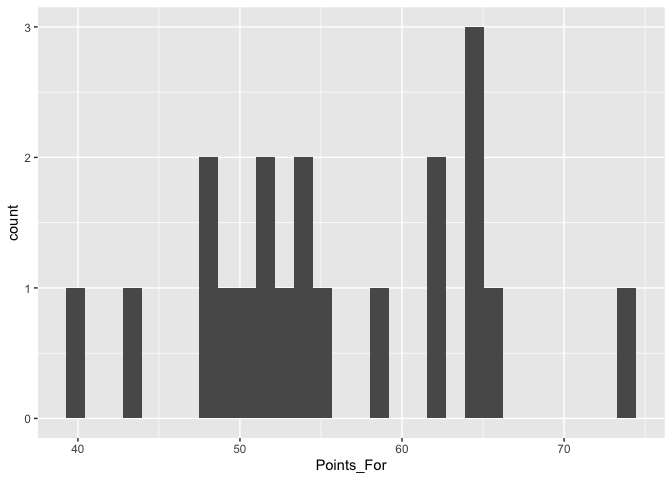
\includegraphics{Introduction_to_Visualizations_for_EDA_files/figure-latex/histogram distribution of points scored by Rivers-1.pdf}

Now let's add some labels to your axes and give the histogram a title.
To start, I copied and pasted the code from above.

\begin{Shaded}
\begin{Highlighting}[]
\NormalTok{points_hist <-}\StringTok{ }\NormalTok{RGVB_team }\OperatorTok
\StringTok{            }\KeywordTok{ggplot}\NormalTok{(}\KeywordTok{aes}\NormalTok{(}\DataTypeTok{x =}\NormalTok{ Points_For)) }\OperatorTok{+}
\StringTok{            }\KeywordTok{geom_histogram}\NormalTok{() }\OperatorTok{+}
\StringTok{            }\KeywordTok{labs}\NormalTok{(}\DataTypeTok{x =} \StringTok{"Points Scored"}\NormalTok{, }\DataTypeTok{y =} \StringTok{"Number of Games"}\NormalTok{, }\DataTypeTok{title =} \StringTok{"Distribution of Points Scored Per Game By Rivers Girls Basketball"}\NormalTok{, }\DataTypeTok{subtitle =} \StringTok{"2018-2019 Season"}\NormalTok{)}
\NormalTok{points_hist}
\end{Highlighting}
\end{Shaded}

\begin{verbatim}
## `stat_bin()` using `bins = 30`. Pick better value with `binwidth`.
\end{verbatim}

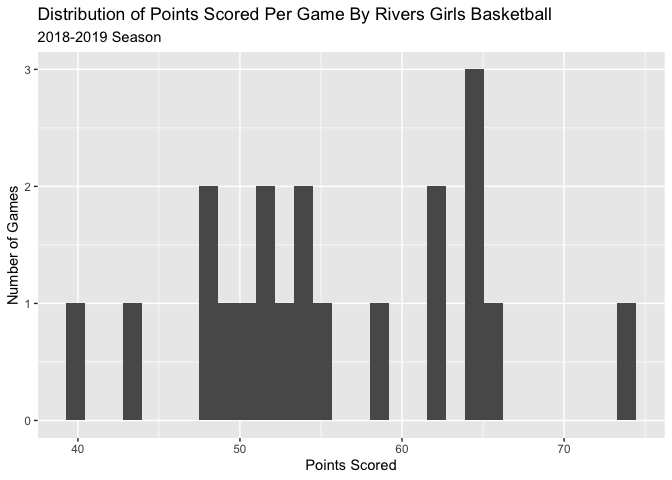
\includegraphics{Introduction_to_Visualizations_for_EDA_files/figure-latex/histogram distribution of points for with labels-1.pdf}

You'll see that a message popped up that says in part ``Pick a better
value with `binwidth'\,'' Let's make that change by adding in bindwith =
10 Reference data visualization principles to make an appropriate
binwidth for your analysis.

\begin{Shaded}
\begin{Highlighting}[]
\NormalTok{points_hist <-}\StringTok{ }\NormalTok{RGVB_team }\OperatorTok
\StringTok{            }\KeywordTok{ggplot}\NormalTok{(}\KeywordTok{aes}\NormalTok{(}\DataTypeTok{x =}\NormalTok{ Points_For)) }\OperatorTok{+}
\StringTok{            }\KeywordTok{geom_histogram}\NormalTok{(}\DataTypeTok{binwidth =} \DecValTok{5}\NormalTok{) }\OperatorTok{+}
\StringTok{            }\KeywordTok{labs}\NormalTok{(}\DataTypeTok{x =} \StringTok{"Points Scored"}\NormalTok{, }\DataTypeTok{y =} \StringTok{"Number of Games"}\NormalTok{, }\DataTypeTok{title =} \StringTok{"Distribution of Points Scored Per Game By Rivers Girls Basketball"}\NormalTok{, }\DataTypeTok{subtitle =} \StringTok{"2018-2019 Season"}\NormalTok{)}
\NormalTok{points_hist}
\end{Highlighting}
\end{Shaded}

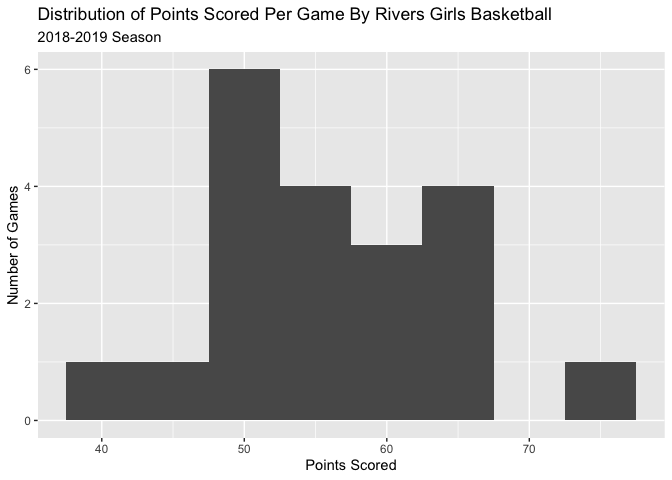
\includegraphics{Introduction_to_Visualizations_for_EDA_files/figure-latex/histogram distribution with new bins-1.pdf}

Now let's change the color and outline of the bars.

\begin{Shaded}
\begin{Highlighting}[]
\NormalTok{points_hist <-}\StringTok{ }\NormalTok{RGVB_team }\OperatorTok
\StringTok{            }\KeywordTok{ggplot}\NormalTok{(}\KeywordTok{aes}\NormalTok{(}\DataTypeTok{x =}\NormalTok{ Points_For)) }\OperatorTok{+}
\StringTok{            }\KeywordTok{geom_histogram}\NormalTok{(}\DataTypeTok{binwidth =} \DecValTok{5}\NormalTok{, }\DataTypeTok{color =} \StringTok{"black"}\NormalTok{, }\DataTypeTok{fill =} \StringTok{"red"}\NormalTok{) }\OperatorTok{+}
\StringTok{            }\KeywordTok{labs}\NormalTok{(}\DataTypeTok{x =} \StringTok{"Points Scored"}\NormalTok{, }\DataTypeTok{y =} \StringTok{"Number of Games"}\NormalTok{, }\DataTypeTok{title =} \StringTok{"Distribution of Points Scored Per Game By Rivers Girls Basketball"}\NormalTok{, }\DataTypeTok{subtitle =} \StringTok{"2018-2019 Season"}\NormalTok{)}
\NormalTok{points_hist}
\end{Highlighting}
\end{Shaded}

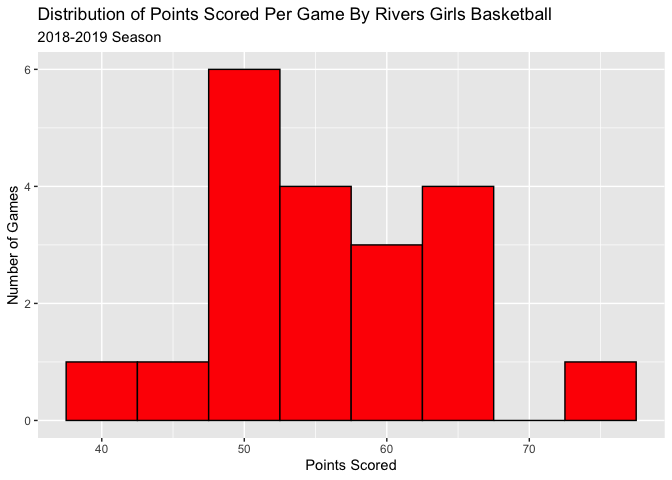
\includegraphics{Introduction_to_Visualizations_for_EDA_files/figure-latex/histogram distribution with style changes-1.pdf}

To finish let's set the scales of the x and y axes, add in a line for
the median, and change the theme to clean things up a bit.

\begin{Shaded}
\begin{Highlighting}[]
\NormalTok{points_hist <-}\StringTok{ }\NormalTok{RGVB_team }\OperatorTok
\StringTok{            }\KeywordTok{ggplot}\NormalTok{(}\KeywordTok{aes}\NormalTok{(}\DataTypeTok{x =}\NormalTok{ Points_For)) }\OperatorTok{+}
\StringTok{            }\KeywordTok{geom_histogram}\NormalTok{(}\DataTypeTok{binwidth =} \DecValTok{5}\NormalTok{, }\DataTypeTok{color =} \StringTok{"white"}\NormalTok{, }\DataTypeTok{fill =} \StringTok{"red"}\NormalTok{) }\OperatorTok{+}
\StringTok{            }\KeywordTok{labs}\NormalTok{(}\DataTypeTok{x =} \StringTok{"Points Scored"}\NormalTok{, }\DataTypeTok{y =} \StringTok{"Number of Games"}\NormalTok{, }
                 \DataTypeTok{title =} \StringTok{"Distribution of Points Scored Per Game By Rivers Girls Basketball"}\NormalTok{, }
                 \DataTypeTok{subtitle =} \StringTok{"2018-2019 Season"}\NormalTok{)  }\OperatorTok{+}
\StringTok{            }\KeywordTok{scale_x_continuous}\NormalTok{(}\DataTypeTok{limits =} \KeywordTok{c}\NormalTok{(}\DecValTok{0}\NormalTok{, }\DecValTok{90}\NormalTok{),}
                     \DataTypeTok{breaks =} \KeywordTok{seq}\NormalTok{(}\DecValTok{0}\NormalTok{, }\DecValTok{90}\NormalTok{, }\DecValTok{10}\NormalTok{))}\OperatorTok{+}
\StringTok{            }\KeywordTok{scale_y_continuous}\NormalTok{(}\DataTypeTok{limits =} \KeywordTok{c}\NormalTok{(}\DecValTok{0}\NormalTok{, }\DecValTok{8}\NormalTok{),}
                     \DataTypeTok{breaks =} \KeywordTok{seq}\NormalTok{(}\DecValTok{0}\NormalTok{, }\DecValTok{8}\NormalTok{, }\DecValTok{1}\NormalTok{)) }\OperatorTok{+}
\StringTok{        }\KeywordTok{geom_vline}\NormalTok{(}\KeywordTok{aes}\NormalTok{(}\DataTypeTok{xintercept =} \KeywordTok{median}\NormalTok{(Points_For)), }\DataTypeTok{color =} \StringTok{"black"}\NormalTok{)  }\OperatorTok{+}
\StringTok{        }\KeywordTok{theme}\NormalTok{(}\DataTypeTok{panel.grid.major =} \KeywordTok{element_blank}\NormalTok{(), }\DataTypeTok{panel.grid.minor =} \KeywordTok{element_blank}\NormalTok{(), }\DataTypeTok{panel.background =} \KeywordTok{element_blank}\NormalTok{())}
            
\NormalTok{points_hist}
\end{Highlighting}
\end{Shaded}

\begin{verbatim}
## Warning: Removed 2 rows containing missing values (geom_bar).
\end{verbatim}

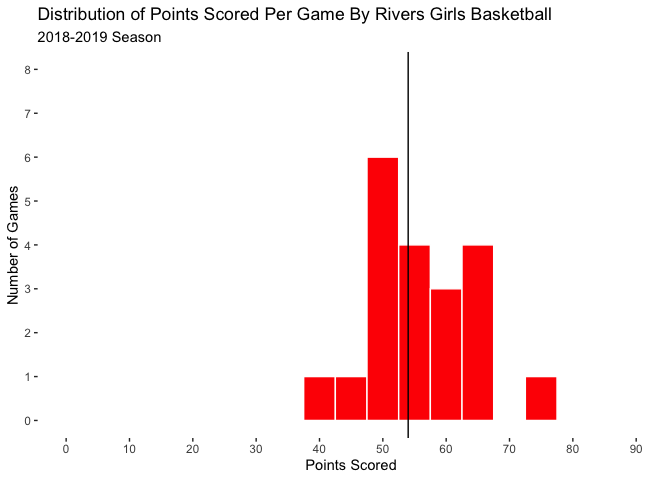
\includegraphics{Introduction_to_Visualizations_for_EDA_files/figure-latex/histogram distribution and median line-1.pdf}

\hypertarget{density-curve}{%
\subsection{Density Curve}\label{density-curve}}

There are times when a density curve will more clearly show the
distribution of quantitative data. Let's say you are going through your
EDA and create a histogram first and realize a density curve would be a
better visualization: - copy and paste your code - change the name -
change geom\_histogram to geom\_density - delete binwidth = - take out
the scales code for the y-axis - change the y-axis label to y = "".

\begin{Shaded}
\begin{Highlighting}[]
\NormalTok{points_density <-}\StringTok{ }\NormalTok{RGVB_team }\OperatorTok
\StringTok{            }\KeywordTok{ggplot}\NormalTok{(}\KeywordTok{aes}\NormalTok{(}\DataTypeTok{x =}\NormalTok{ Points_For)) }\OperatorTok{+}
\StringTok{            }\KeywordTok{geom_density}\NormalTok{(}\DataTypeTok{color =} \StringTok{"white"}\NormalTok{, }\DataTypeTok{fill =} \StringTok{"red"}\NormalTok{) }\OperatorTok{+}
\StringTok{            }\KeywordTok{labs}\NormalTok{(}\DataTypeTok{x =} \StringTok{"Points Scored"}\NormalTok{, }\DataTypeTok{y =} \StringTok{""}\NormalTok{, }
                 \DataTypeTok{title =} \StringTok{"Distribution of Points Scored Per Game By Rivers Girls Basketball"}\NormalTok{, }
                 \DataTypeTok{subtitle =} \StringTok{"2018-2019 Season"}\NormalTok{)  }\OperatorTok{+}
\StringTok{            }\KeywordTok{scale_x_continuous}\NormalTok{(}\DataTypeTok{limits =} \KeywordTok{c}\NormalTok{(}\DecValTok{0}\NormalTok{, }\DecValTok{90}\NormalTok{),}
                     \DataTypeTok{breaks =} \KeywordTok{seq}\NormalTok{(}\DecValTok{0}\NormalTok{, }\DecValTok{90}\NormalTok{, }\DecValTok{10}\NormalTok{)) }\OperatorTok{+}
\StringTok{        }\KeywordTok{geom_vline}\NormalTok{(}\KeywordTok{aes}\NormalTok{(}\DataTypeTok{xintercept =} \KeywordTok{median}\NormalTok{(Points_For)), }\DataTypeTok{color =} \StringTok{"black"}\NormalTok{)  }\OperatorTok{+}
\StringTok{        }\KeywordTok{theme}\NormalTok{(}\DataTypeTok{panel.grid.major =} \KeywordTok{element_blank}\NormalTok{(), }\DataTypeTok{panel.grid.minor =} \KeywordTok{element_blank}\NormalTok{(), }\DataTypeTok{panel.background =} \KeywordTok{element_blank}\NormalTok{())}
            
\NormalTok{points_density }
\end{Highlighting}
\end{Shaded}

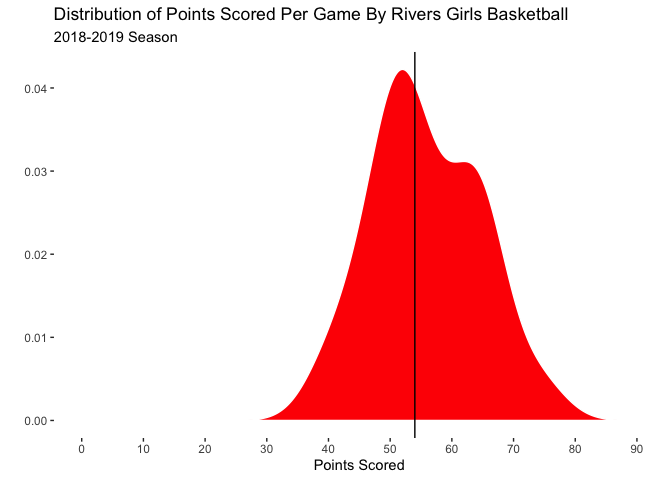
\includegraphics{Introduction_to_Visualizations_for_EDA_files/figure-latex/Density Curves for distribution-1.pdf}

\hypertarget{box-plots}{%
\subsection{Box Plots}\label{box-plots}}

Box plots are great for comparing distributions. Let's use them to
compare the points scored during home games vs away games.

\begin{Shaded}
\begin{Highlighting}[]
\NormalTok{points_HVA_boxes <-}\StringTok{ }\NormalTok{RGVB_team }\OperatorTok
\StringTok{            }\KeywordTok{ggplot}\NormalTok{(}\KeywordTok{aes}\NormalTok{(}\DataTypeTok{x =}\NormalTok{ H_V_A , }\DataTypeTok{y =}\NormalTok{ Points_For)) }\OperatorTok{+}
\StringTok{            }\KeywordTok{geom_boxplot}\NormalTok{() }\OperatorTok{+}
\StringTok{            }\KeywordTok{theme_classic}\NormalTok{()}
\NormalTok{points_HVA_boxes}
\end{Highlighting}
\end{Shaded}

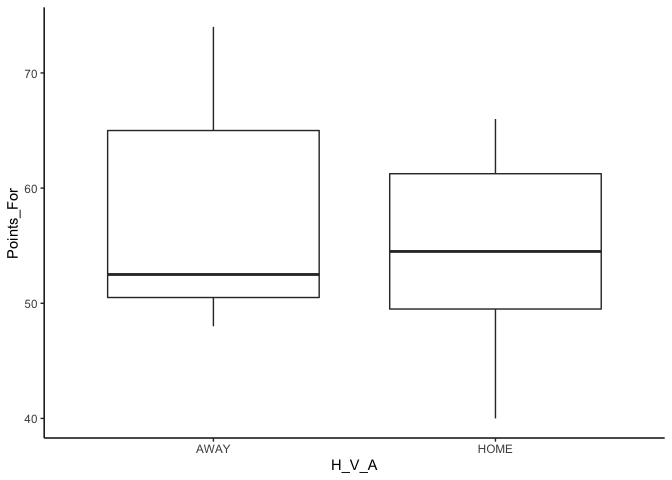
\includegraphics{Introduction_to_Visualizations_for_EDA_files/figure-latex/Box Plots to Compare Distributions-1.pdf}

Before adding any style changes to this visualization, we want to make
it easier for our reader to make conclusions. Therefore, we want to
reorder these boxes from the greatest median to the least. To see this
change, look at how code after aes changed.

I also added in some code to change the style. Try to figure out what
each addition changed.

\begin{Shaded}
\begin{Highlighting}[]
\NormalTok{points_HVA_boxes <-}\StringTok{ }\NormalTok{RGVB_team }\OperatorTok
\StringTok{            }\KeywordTok{ggplot}\NormalTok{(}\KeywordTok{aes}\NormalTok{(}\DataTypeTok{x =} \KeywordTok{reorder}\NormalTok{(H_V_A, Points_For, }\DataTypeTok{.desc =} \OtherTok{TRUE}\NormalTok{), }\DataTypeTok{y =}\NormalTok{ Points_For, }\DataTypeTok{color =}\NormalTok{ H_V_A)) }\OperatorTok{+}
\StringTok{            }\KeywordTok{geom_boxplot}\NormalTok{() }\OperatorTok{+}
\StringTok{            }\KeywordTok{geom_jitter}\NormalTok{(}\DataTypeTok{alpha =} \FloatTok{0.3}\NormalTok{) }\OperatorTok{+}
\StringTok{            }\KeywordTok{scale_color_manual}\NormalTok{(}\DataTypeTok{values =} \KeywordTok{c}\NormalTok{(}\StringTok{"black"}\NormalTok{, }\StringTok{"red"}\NormalTok{)) }\OperatorTok{+}
\StringTok{            }\KeywordTok{labs}\NormalTok{(}\DataTypeTok{title =} \StringTok{"Distribution of Points Scored by Rivers Girls Basketball During Home and Away"}\NormalTok{, }\DataTypeTok{subtitle =} \StringTok{"2018-2019 Season"}\NormalTok{, }\DataTypeTok{x =} \StringTok{""}\NormalTok{, }\DataTypeTok{y =} \StringTok{"Points Scored"}\NormalTok{, }\DataTypeTok{color =} \StringTok{""}\NormalTok{) }\OperatorTok{+}
\StringTok{            }\KeywordTok{theme_classic}\NormalTok{()}
\NormalTok{points_HVA_boxes}
\end{Highlighting}
\end{Shaded}

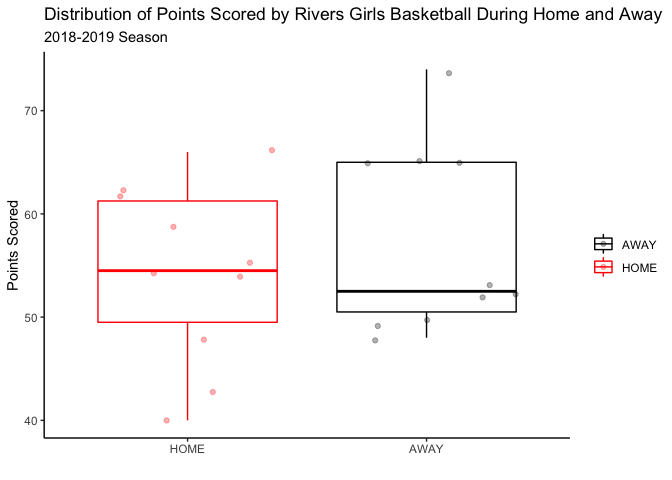
\includegraphics{Introduction_to_Visualizations_for_EDA_files/figure-latex/Box Plots to Compare Distributions reorder-1.pdf}

Sometimes box plots are easier to read when they are stacked on top of
one another. Use coord\_flip to do that. Let's also add in labels while
we are here. You will do that using the labs code like you did when
making the histograms and density curves.

\begin{Shaded}
\begin{Highlighting}[]
\NormalTok{flip_points_HVA_boxes <-}\StringTok{ }\NormalTok{RGVB_team }\OperatorTok
\StringTok{            }\KeywordTok{ggplot}\NormalTok{(}\KeywordTok{aes}\NormalTok{(}\DataTypeTok{x =} \KeywordTok{reorder}\NormalTok{(H_V_A, Points_For, }\DataTypeTok{.desc =} \OtherTok{TRUE}\NormalTok{), }\DataTypeTok{y =}\NormalTok{ Points_For, }\DataTypeTok{color =}\NormalTok{ H_V_A)) }\OperatorTok{+}
\StringTok{            }\KeywordTok{geom_boxplot}\NormalTok{() }\OperatorTok{+}
\StringTok{            }\KeywordTok{geom_jitter}\NormalTok{(}\DataTypeTok{alpha =} \FloatTok{0.3}\NormalTok{) }\OperatorTok{+}
\StringTok{            }\KeywordTok{scale_color_manual}\NormalTok{(}\DataTypeTok{values =} \KeywordTok{c}\NormalTok{(}\StringTok{"black"}\NormalTok{, }\StringTok{"red"}\NormalTok{)) }\OperatorTok{+}
\StringTok{            }\KeywordTok{labs}\NormalTok{(}\DataTypeTok{title =} \StringTok{"Distribution of Points Scored by Rivers Girls Basketball During Home and Away"}\NormalTok{, }\DataTypeTok{subtitle =} \StringTok{"2018-2019 Season"}\NormalTok{, }\DataTypeTok{x =} \StringTok{""}\NormalTok{, }\DataTypeTok{y =} \StringTok{"Points Scored"}\NormalTok{, }\DataTypeTok{color =} \StringTok{""}\NormalTok{) }\OperatorTok{+}
\StringTok{            }\KeywordTok{theme_classic}\NormalTok{() }\OperatorTok{+}
\StringTok{            }\KeywordTok{coord_flip}\NormalTok{()}
\NormalTok{flip_points_HVA_boxes}
\end{Highlighting}
\end{Shaded}

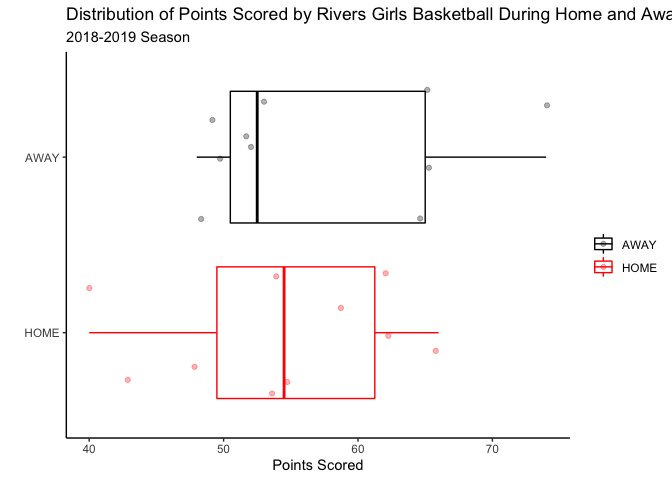
\includegraphics{Introduction_to_Visualizations_for_EDA_files/figure-latex/Box Plots to Compare Distributions add titles and flip-1.pdf}

\hypertarget{bar-plots}{%
\subsection{Bar Plots}\label{bar-plots}}

We'll use the bar plot to visualize categorical data. In this first
example, we will look at the marginal distribution of result. In other
words, the heights of the bars will represent the number of games they
won and lost.

\begin{Shaded}
\begin{Highlighting}[]
\NormalTok{wl_bars <-}\StringTok{ }\NormalTok{RGVB_team }\OperatorTok
\StringTok{          }\KeywordTok{ggplot}\NormalTok{(}\KeywordTok{aes}\NormalTok{(}\DataTypeTok{x =}\NormalTok{ Result)) }\OperatorTok{+}
\StringTok{          }\KeywordTok{geom_bar}\NormalTok{()}
\NormalTok{wl_bars}
\end{Highlighting}
\end{Shaded}

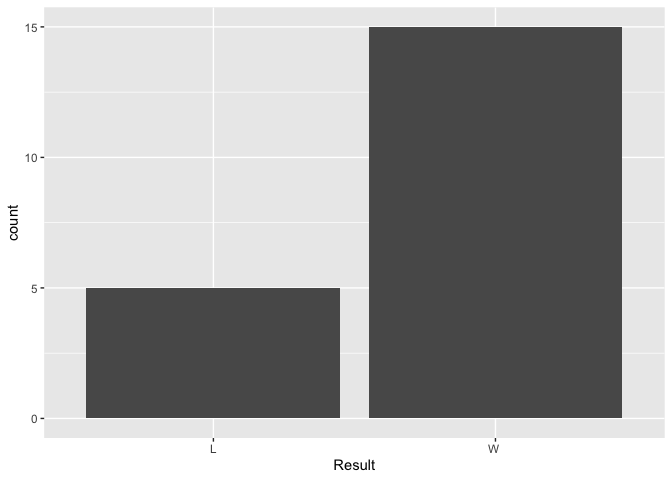
\includegraphics{Introduction_to_Visualizations_for_EDA_files/figure-latex/Bar plot basic-1.pdf}

Because we would most likely want to highlight the largest bar, let's
put that one first. To do this, we have to change the order of the bars
to go from greatest to least.

Let's start by making a table using the skills we learned in previous
activities to see the number of games for each result. After, we will
use that data frame to make our bar plot.

In this example, I have not made changes to the style. Knowing how style
changes were made to previous visualizations, try to make similar
changes to this one. If you are confused, start by changing the title
and axes labels.

\begin{Shaded}
\begin{Highlighting}[]
\NormalTok{wl_count <-}\StringTok{ }\NormalTok{RGVB_team }\OperatorTok
\StringTok{            }\KeywordTok{group_by}\NormalTok{(Result) }\OperatorTok
\StringTok{            }\KeywordTok{summarize}\NormalTok{(}\DataTypeTok{count =} \KeywordTok{n}\NormalTok{()) }\OperatorTok
\StringTok{            }\KeywordTok{arrange}\NormalTok{(}\KeywordTok{desc}\NormalTok{(count))}
\NormalTok{wl_count}
\end{Highlighting}
\end{Shaded}

\begin{verbatim}
## # A tibble: 2 x 2
##   Result count
##   <fct>  <int>
## 1 "W "      15
## 2 L          5
\end{verbatim}

\begin{Shaded}
\begin{Highlighting}[]
\NormalTok{wl_bar_order <-}\StringTok{ }\NormalTok{wl_count }\OperatorTok
\StringTok{          }\KeywordTok{ggplot}\NormalTok{(}\KeywordTok{aes}\NormalTok{(}\DataTypeTok{x =} \KeywordTok{reorder}\NormalTok{(Result, }\OperatorTok{-}\NormalTok{count), }\DataTypeTok{y =}\NormalTok{ count)) }\OperatorTok{+}
\StringTok{          }\KeywordTok{geom_bar}\NormalTok{(}\DataTypeTok{stat =} \StringTok{'identity'}\NormalTok{)}
\NormalTok{wl_bar_order}
\end{Highlighting}
\end{Shaded}

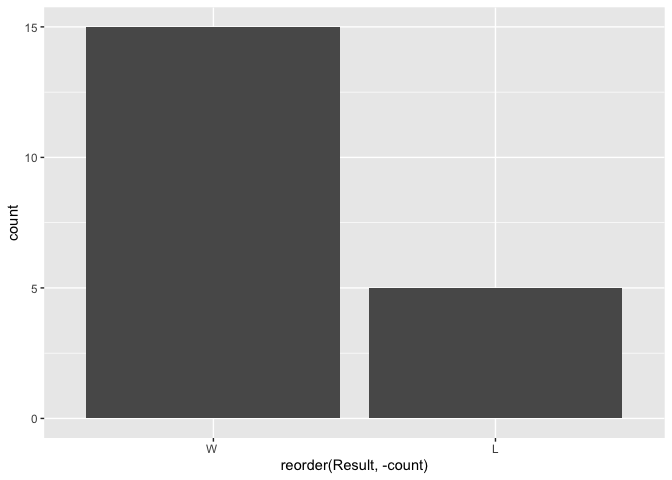
\includegraphics{Introduction_to_Visualizations_for_EDA_files/figure-latex/Bar plot ordering bars-1.pdf}

\hypertarget{stacked-bar-graph}{%
\subsection{100\% Stacked Bar Graph}\label{stacked-bar-graph}}

When you want to examine conditional distributions, a good option is a
100\% stacked bar graph. For this example, we want to look at the
proportion of home games and away games were won i.e., You will be able
to answer the question, ``Did they win a higher percentage of games at
home or away?'' It's important to remember that you use this when
studying two categorical variables.

\begin{Shaded}
\begin{Highlighting}[]
\NormalTok{wl_venue <-}\StringTok{ }\NormalTok{RGVB_team }\OperatorTok
\StringTok{            }\KeywordTok{ggplot}\NormalTok{(}\KeywordTok{aes}\NormalTok{(H_V_A, }\DataTypeTok{fill =}\NormalTok{ Result)) }\OperatorTok{+}
\StringTok{            }\KeywordTok{geom_bar}\NormalTok{(}\DataTypeTok{position =} \StringTok{"fill"}\NormalTok{) }\OperatorTok{+}
\StringTok{            }\KeywordTok{labs}\NormalTok{(}\DataTypeTok{x =} \StringTok{""}\NormalTok{, }\DataTypeTok{y =} \StringTok{"Proportion"}\NormalTok{, }\DataTypeTok{fill =} \StringTok{""}\NormalTok{) }\OperatorTok{+}
\StringTok{        }\KeywordTok{theme}\NormalTok{(}\DataTypeTok{panel.grid.major =} \KeywordTok{element_blank}\NormalTok{(), }\DataTypeTok{panel.grid.minor =} \KeywordTok{element_blank}\NormalTok{(), }\DataTypeTok{panel.background =} \KeywordTok{element_blank}\NormalTok{())}
\NormalTok{wl_venue}
\end{Highlighting}
\end{Shaded}

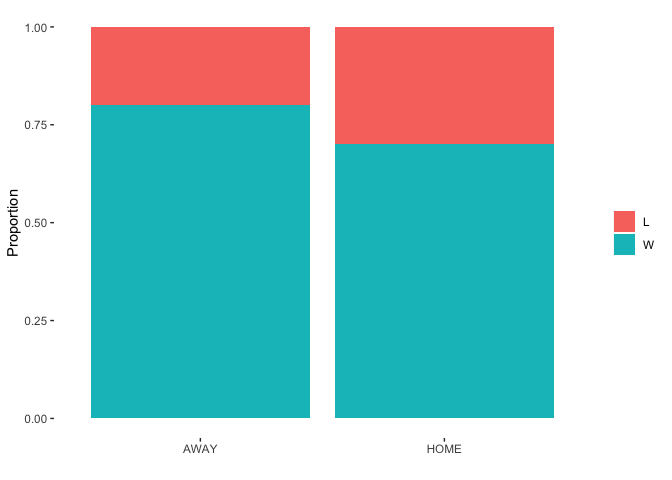
\includegraphics{Introduction_to_Visualizations_for_EDA_files/figure-latex/100 stacked-1.pdf}


\end{document}
